\documentclass{beamer}
\usepackage[utf8]{inputenc}

\usetheme{Madrid}
\usecolortheme{default}
\usepackage{amsmath,amssymb,amsfonts,amsthm}
\usepackage{txfonts}
\usepackage{tkz-euclide}
\usepackage{listings}
\usepackage{adjustbox}
\usepackage{array}
\usepackage{tabularx}
\usepackage{gvv}
\usepackage{lmodern}
\usepackage{circuitikz}
\usepackage{tikz}
\usepackage{graphicx}

\setbeamertemplate{page number in head/foot}[totalframenumber]

\usepackage{tcolorbox}
\tcbuselibrary{minted,breakable,xparse,skins}



\definecolor{bg}{gray}{0.95}
\DeclareTCBListing{mintedbox}{O{}m!O{}}{%
  breakable=true,
  listing engine=minted,
  listing only,
  minted language=#2,
  minted style=default,
  minted options={%
    linenos,
    gobble=0,
    breaklines=true,
    breakafter=,,
    fontsize=\small,
    numbersep=8pt,
    #1},
  boxsep=0pt,
  left skip=0pt,
  right skip=0pt,
  left=25pt,
  right=0pt,
  top=3pt,
  bottom=3pt,
  arc=5pt,
  leftrule=0pt,
  rightrule=0pt,
  bottomrule=2pt,

  colback=bg,
  colframe=orange!70,
  enhanced,
  overlay={%
    \begin{tcbclipinterior}
    \fill[orange!20!white] (frame.south west) rectangle ([xshift=20pt]frame.north west);
    \end{tcbclipinterior}},
  #3,
}
\lstset{
    language=C,
    basicstyle=\ttfamily\small,
    keywordstyle=\color{blue},
    stringstyle=\color{orange},
    commentstyle=\color{green!60!black},
    numbers=left,
    numberstyle=\tiny\color{gray},
    breaklines=true,
    showstringspaces=false,
}
%------------------------------------------------------------
%This block of code defines the information to appear in the
%Title page
\title %optional
{1.10.24}
\date{September 2025}
%\subtitle{A short story}

\author % (optional)
{Tangellapalli Mohana Krishna Sushma - EE25BTECH11058}



\begin{document}

\frame{\titlepage}
\begin{frame}{Question}
 Find the direction cosines of the unit vector perpendicular to the plane
\begin{align*}
    \vec{r} \cdot (6\hat{\imath} - 3\hat{\jmath} - 2\hat{k}) + 1 = 0
\end{align*}
\hspace{1cm}passing through the origin.


\end{frame}

\begin{frame}{given data}

The plane equation:
\begin{align*}
\vec{r} \cdot (6\vec{i} - 3\vec{j} - 2\vec{k}) + 1 = 0
\end{align*}

The normal vector to the plane:
\begin{align*}
\vec{n} = \begin{pmatrix} 6 \\ -3 \\ -2 \end{pmatrix}
\end{align*}
\end{frame}

\begin{frame}{Formula}

To find the unit vector perpendicular to the plane:

\begin{align*}
\vec{u} = \frac{1}{\|\vec{n}\|} \vec{n}
\end{align*}

where $\vec{n}$ is the normal vector of the plane.

\end{frame}

Norm of the vector $\vec{n}$,
\begin{align}
    \vec{u} = \frac{1}{\|\vec{n}\|} \vec{n} 
    = \frac{1}{7}
    \begin{pmatrix}
        6 \\[2pt]
        -3 \\[2pt]
        -2
    \end{pmatrix}
    =
    \begin{pmatrix}
        \dfrac{6}{7} \\[2pt]
        -\dfrac{3}{7} \\[2pt]
        -\dfrac{2}{7}
    \end{pmatrix}
\end{align}


The direction cosines of the unit vector perpendicular to the plane are 
\[
    \left(
        \frac{6}{7},\;
        -\frac{3}{7},\;
        -\frac{2}{7}
    \right)
\]


\begin{frame}[fragile]
    \frametitle{Python Code}
    \begin{lstlisting}
import numpy as np
import matplotlib.pyplot as plt
from mpl_toolkits.mplot3d import Axes3D

# Define the plane: 6x - 3y - 2z + 1 = 0
normal = np.array([6, -3, -2])  # Normal vector to the plane

# Create grid for the plane
x = np.linspace(-5, 5, 10)
y = np.linspace(-5, 5, 10)
X, Y = np.meshgrid(x, y)
Z = (6*X - 3*Y + 1)/2  # Rearranged plane equation

     \end{lstlisting}
\end{frame}


\begin{frame}[fragile]
    \frametitle{Python Code}
    \begin{lstlisting}

    # Plot the plane
fig = plt.figure(figsize=(10, 8))
ax = fig.add_subplot(111, projection='3d')
ax.plot_surface(X, Y, Z, alpha=0.5, color='cyan', edgecolor='k')

# Plot the normal vector from the origin
ax.quiver(0, 0, 0, normal[0], normal[1], normal[2], 
          color='r', linewidth=2, label='Normal Vector (6, -3, -2)')

     \end{lstlisting}
\end{frame}


\begin{frame}[fragile]
    \frametitle{Python Code}
    \begin{lstlisting}

   # Labels
ax.set_xlabel('X-axis')
ax.set_ylabel('Y-axis')
ax.set_zlabel('Z-axis')
ax.set_title('Plane $6x - 3y - 2z + 1 = 0$ and its Normal Vector')

# Legend
ax.legend()

# Show plot
plt.show()

     \end{lstlisting}
\end{frame}

\begin{frame}[fragile]
\frametitle{C Code}
\begin{lstlisting}

#include <stdio.h>
#include <math.h>

int main() {
    // Plane equation: 6x - 3y - 2z + 1 = 0
    // Normal vector = (6, -3, -2)
    double a = 6, b = -3, c = -2;

    // Step 1: Print normal vector
    printf("Normal vector to the plane: (%.2f, %.2f, %.2f)\n", a, b, c);

    // Step 2: Find norm of the vector
    double norm = sqrt(a*a + b*b + c*c);
    printf("Norm of the vector = sqrt(%.2f^2 + %.2f^2 + %.2f^2) = %.2f\n", a, b, c, norm);

    // Step 3: Find unit vector
    double ux = a / norm;
    double uy = b / norm;
    double uz = c / norm;

    printf("Unit vector (u) = (%.2f, %.2f, %.2f)\n", ux, uy, uz);

    // Step 4: Direction cosines = components of unit vector
    printf("Direction cosines of the unit vector perpendicular to the plane:\n");
    printf("l = %.2f, m = %.2f, n = %.2f\n", ux, uy, uz);

    return 0;
}


\end{lstlisting}

\end{frame}

\begin{frame}[fragile]
\frametitle{Python and C Code}

\begin{lstlisting}

import subprocess

# 1. Compile the C program
subprocess.run(["gcc", "direction cosines.c", "-o", "direction cosines"])

# 2. Run the compiled C program
result = subprocess.run(["./direction cosines"], capture_output=True, text=True)

# 3. Print the output from the C program
print(result.stdout)


\end{lstlisting}

\end{frame}

\begin{figure}
    \centering
    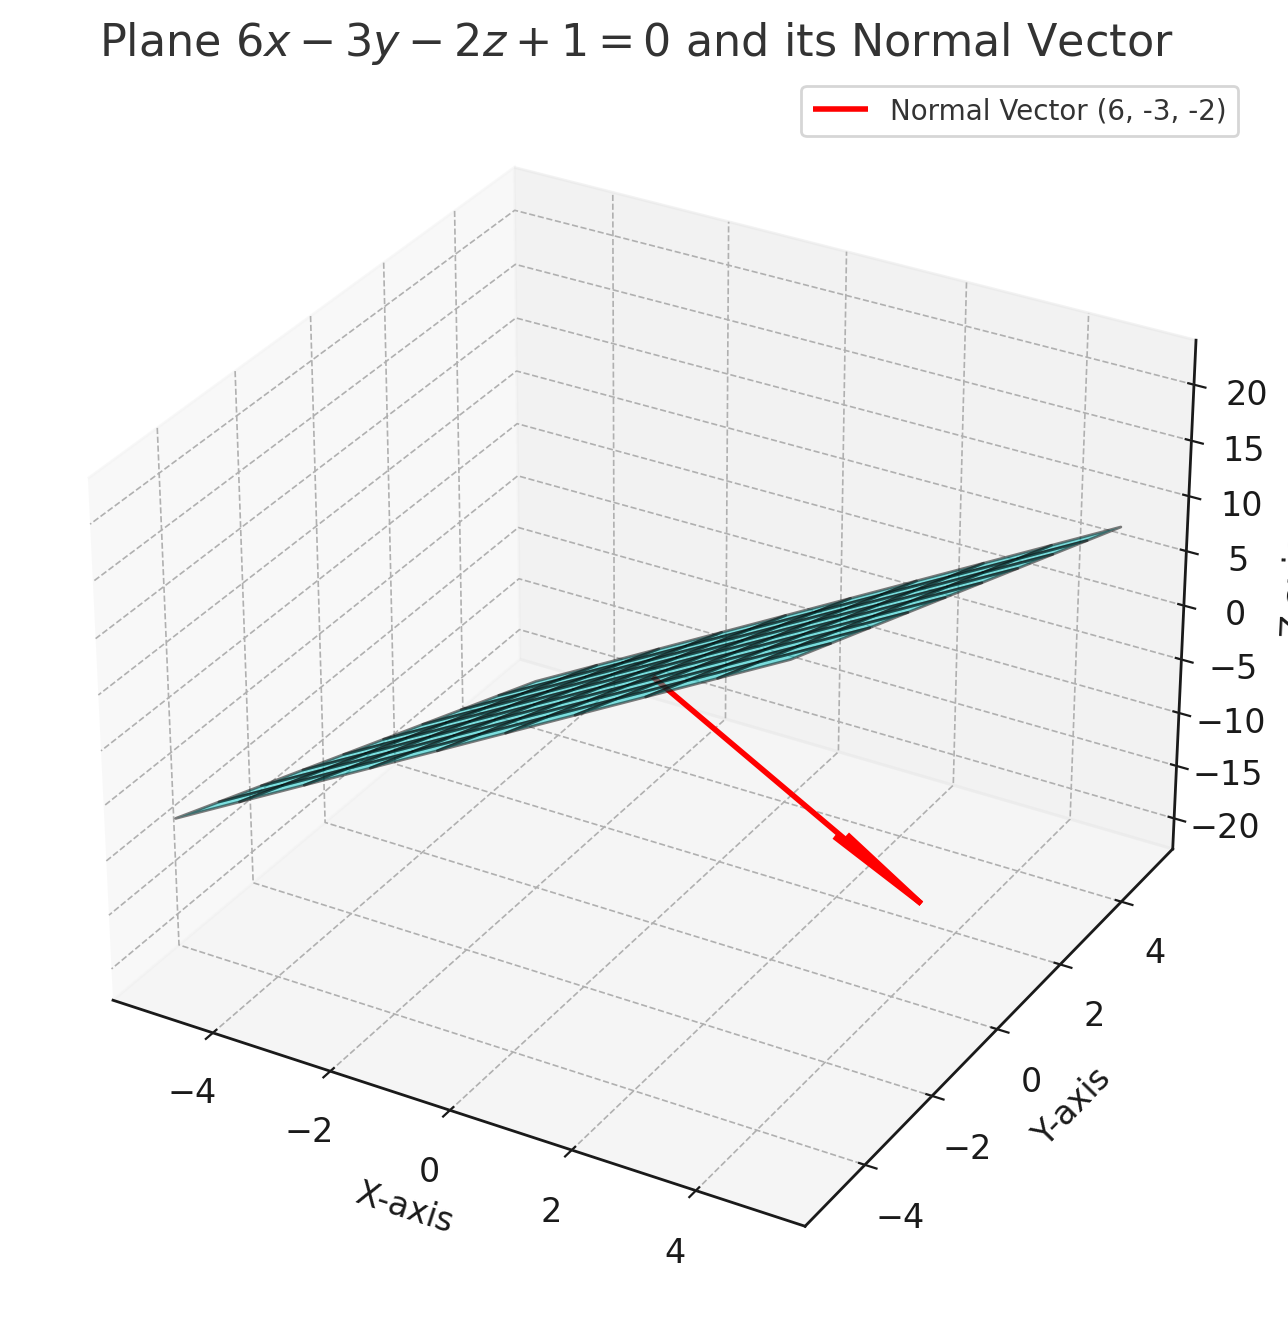
\includegraphics[width=0.8\columnwidth]{figs/fig.png}
    \caption{Plane with Perpendicular Normal Vector}
    \label{fig:placeholder}
\end{figure}

\end{document}